\section{Results}

\subsection{Prototype Capabilities}
The completed system provides several key capabilities. A dashboard aggregates time-series data for different Notion features, displaying interest trajectories over the analysis period. Side-by-side comparisons of the three forecasting models are presented with confidence bands indicating prediction certainty. A recommendation engine translates forecast values into prioritized suggestions regarding which features warrant increased attention and which may require strategic reconsideration. Export functionality enables users to download data in CSV or JSON formats for independent analysis.

\subsection{Forecasting Findings}
Application of the models to Notion feature data revealed several notable patterns.

\textbf{Notion AI} exhibits a clear upward trajectory. Search frequency continues to increase, and review sentiment reflects substantial user interest. Exponential Smoothing captured recent accelerations rapidly, while ARIMA confirmed sustained momentum rather than temporary fluctuation.

\textbf{Templates} demonstrate consistent baseline demand. Interest remains stable without substantial volatility, showing predictable seasonal patterns. Users appear to rely on template functionality as a core platform component.

\textbf{Automation features} exhibit gradual growth. Linear Regression analysis indicated that automation interest correlates with broader trends in the productivity software industry—increased general discussion of workflow automation corresponds to increased Notion automation interest.

\begin{figure}[htbp]
\centering
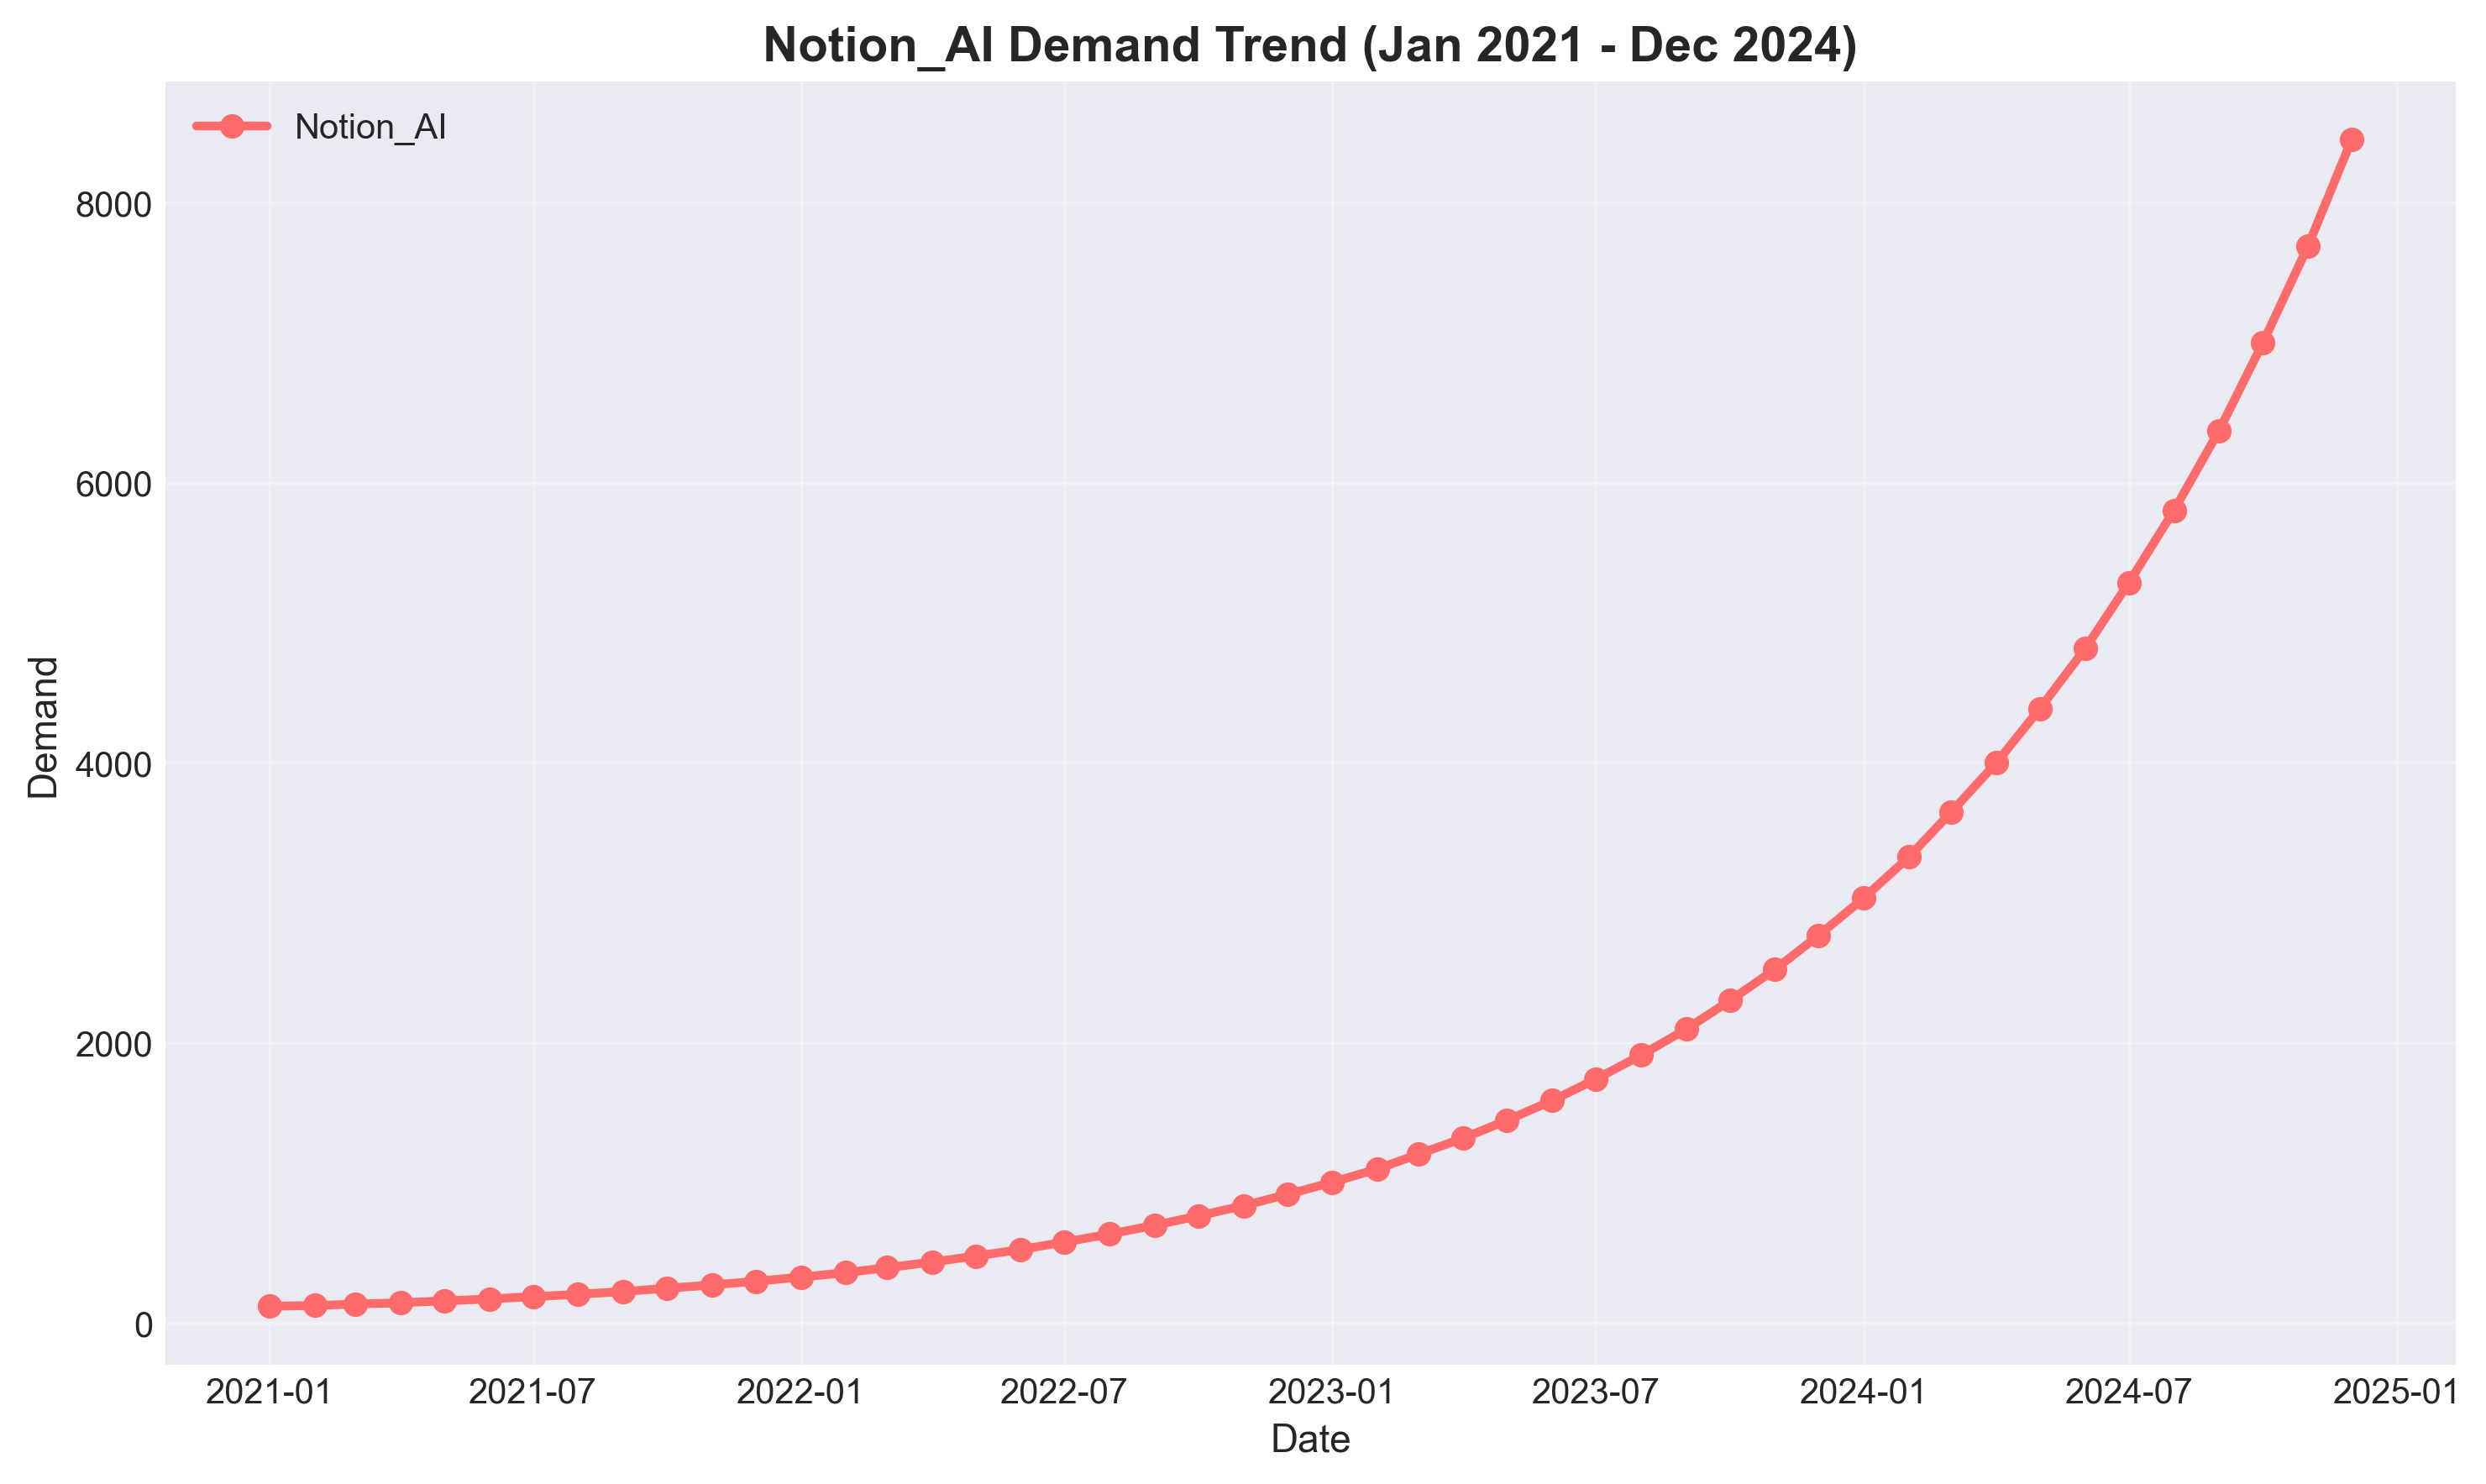
\includegraphics[width=\columnwidth]{figures/fig1a_notion_ai_trend.png}
\caption{Notion AI feature demand trend demonstrating exponential growth from January 2021 to December 2024, with demand increasing from approximately 100 to over 8000. This represents the most substantial growth pattern among all analyzed features.}
\label{fig:ai_trend}
\end{figure}

\begin{figure}[htbp]
\centering
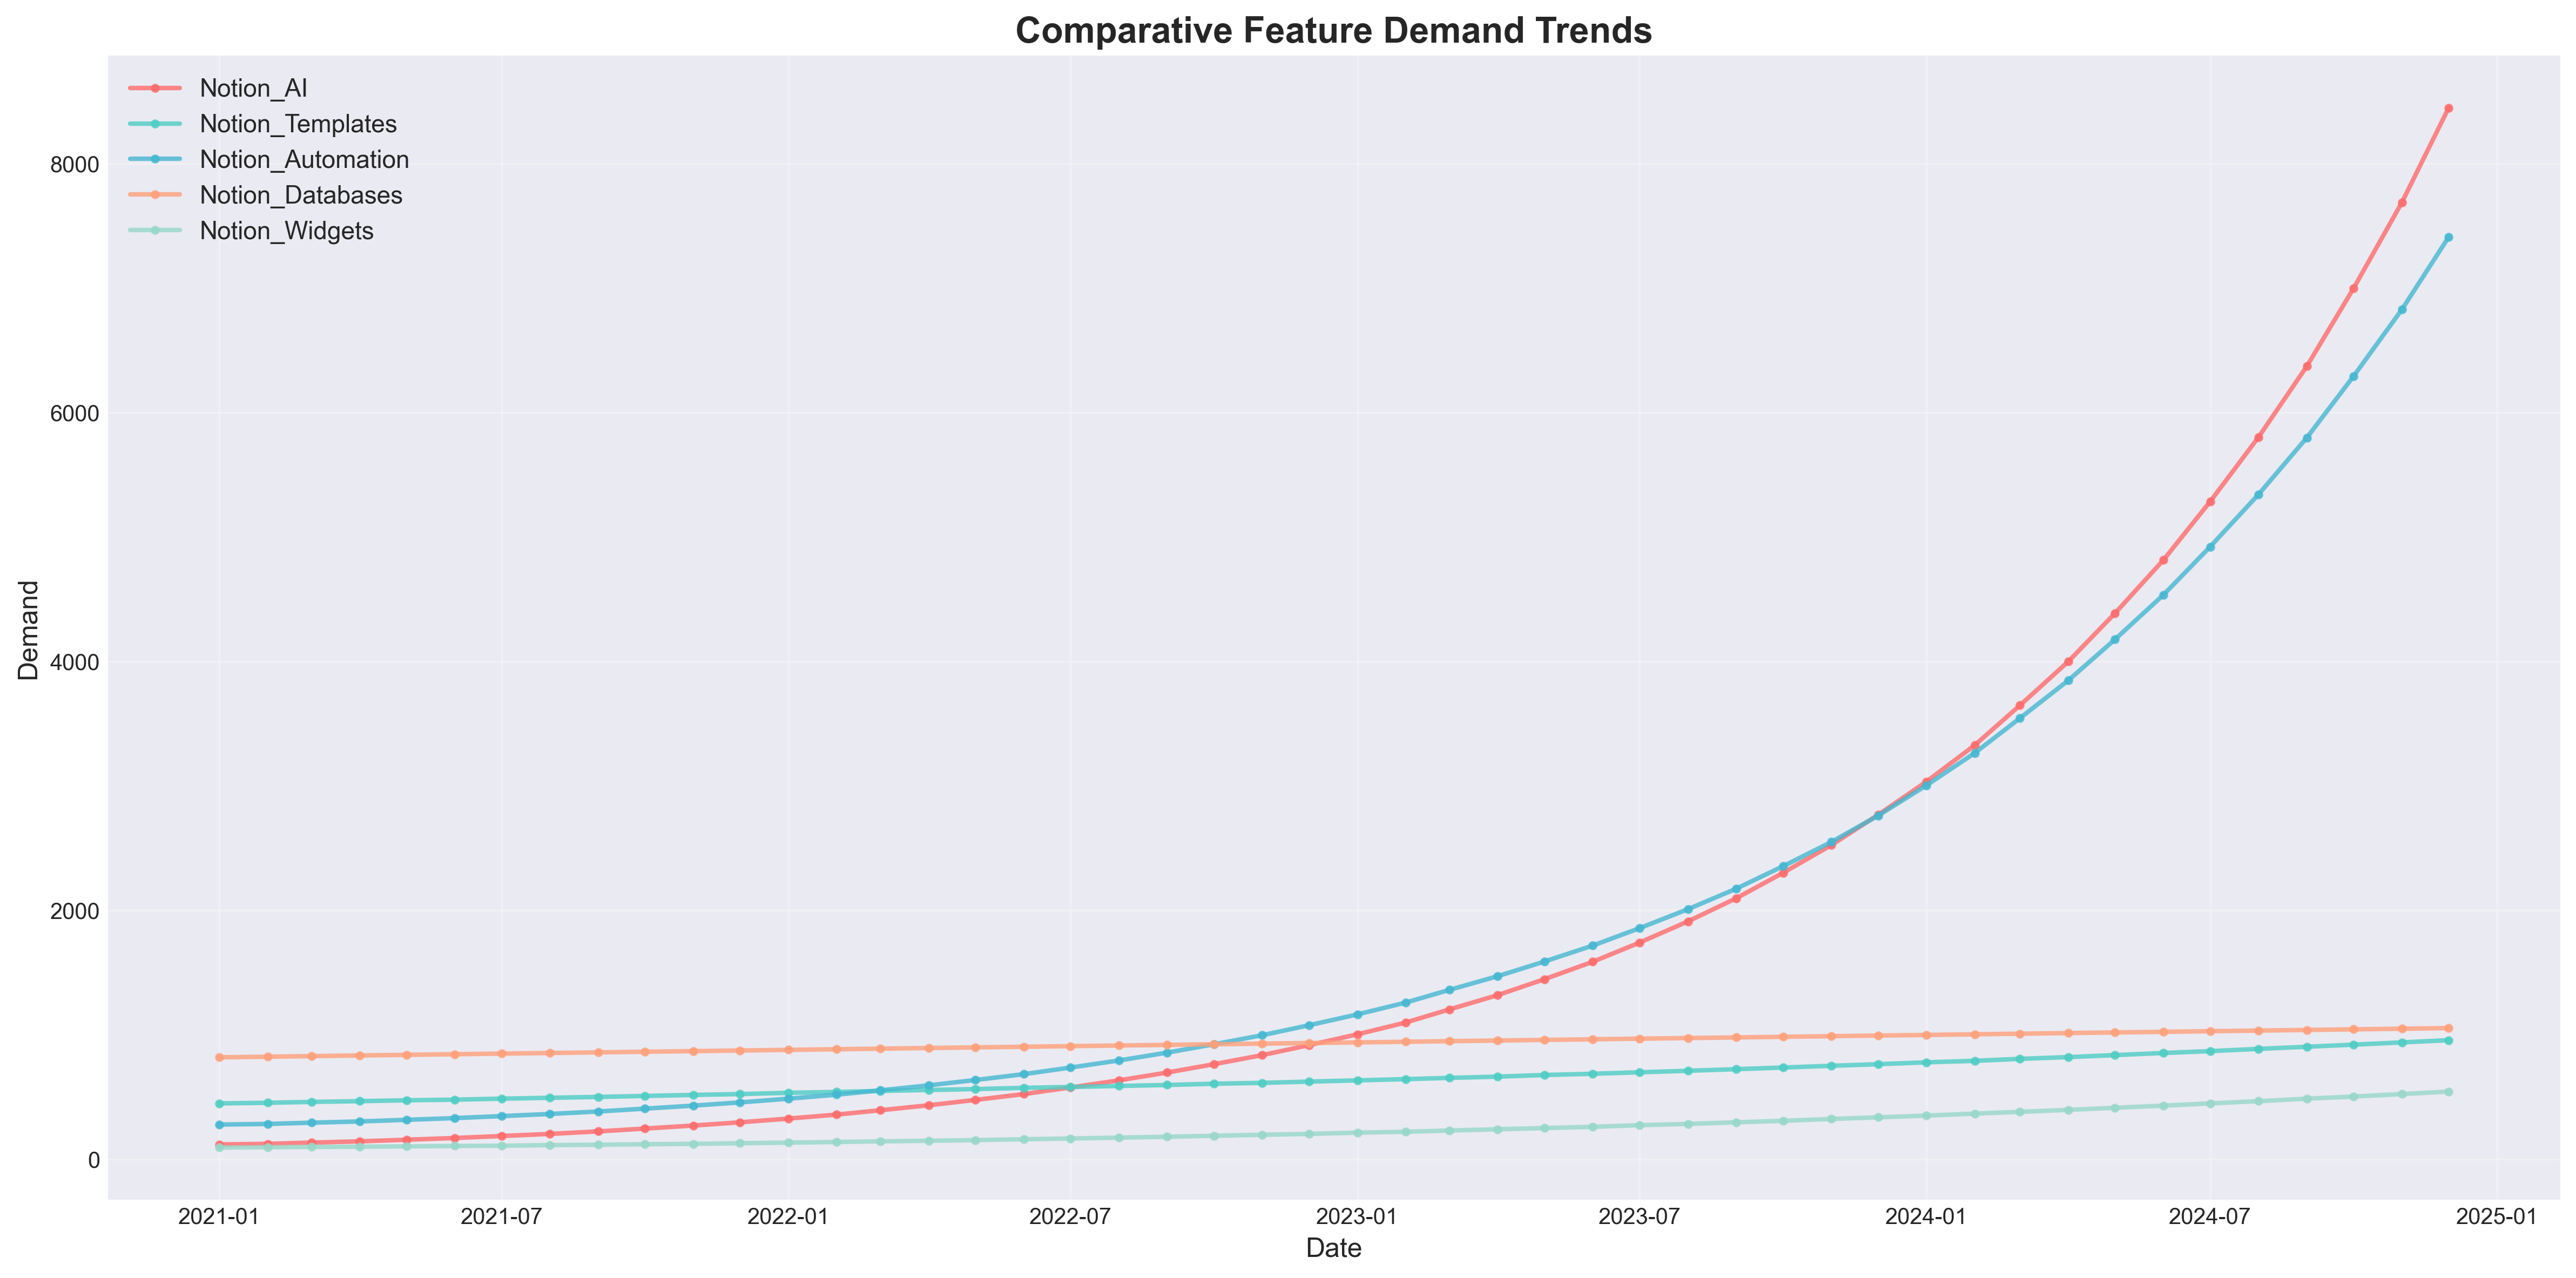
\includegraphics[width=\columnwidth]{figures/fig2_comparative_feature_trends.png}
\caption{Comparative analysis of all feature demands. Notion AI demonstrates dominant growth potential, Templates exhibit steady demand, Automation shows moderate growth, and Databases/Widgets remain stable. This visualization provides insights for resource allocation decisions.}
\label{fig:comparative_trends}
\end{figure}

The ensemble approach combining all three models yielded more reliable predictions than any individual method. The ensemble methodology attenuated the idiosyncrasies of each model.

Figure \ref{fig:ai_trend} illustrates the substantial growth in Notion AI demand, while Figure \ref{fig:comparative_trends} overlays all features on a single chart for relative performance comparison. As shown in Figure \ref{fig:forecast_comparison}, each forecasting method produces slightly different predictions, but all three converge on the fundamental trend: continued strong growth in Notion AI demand.

\begin{figure}[htbp]
\centering
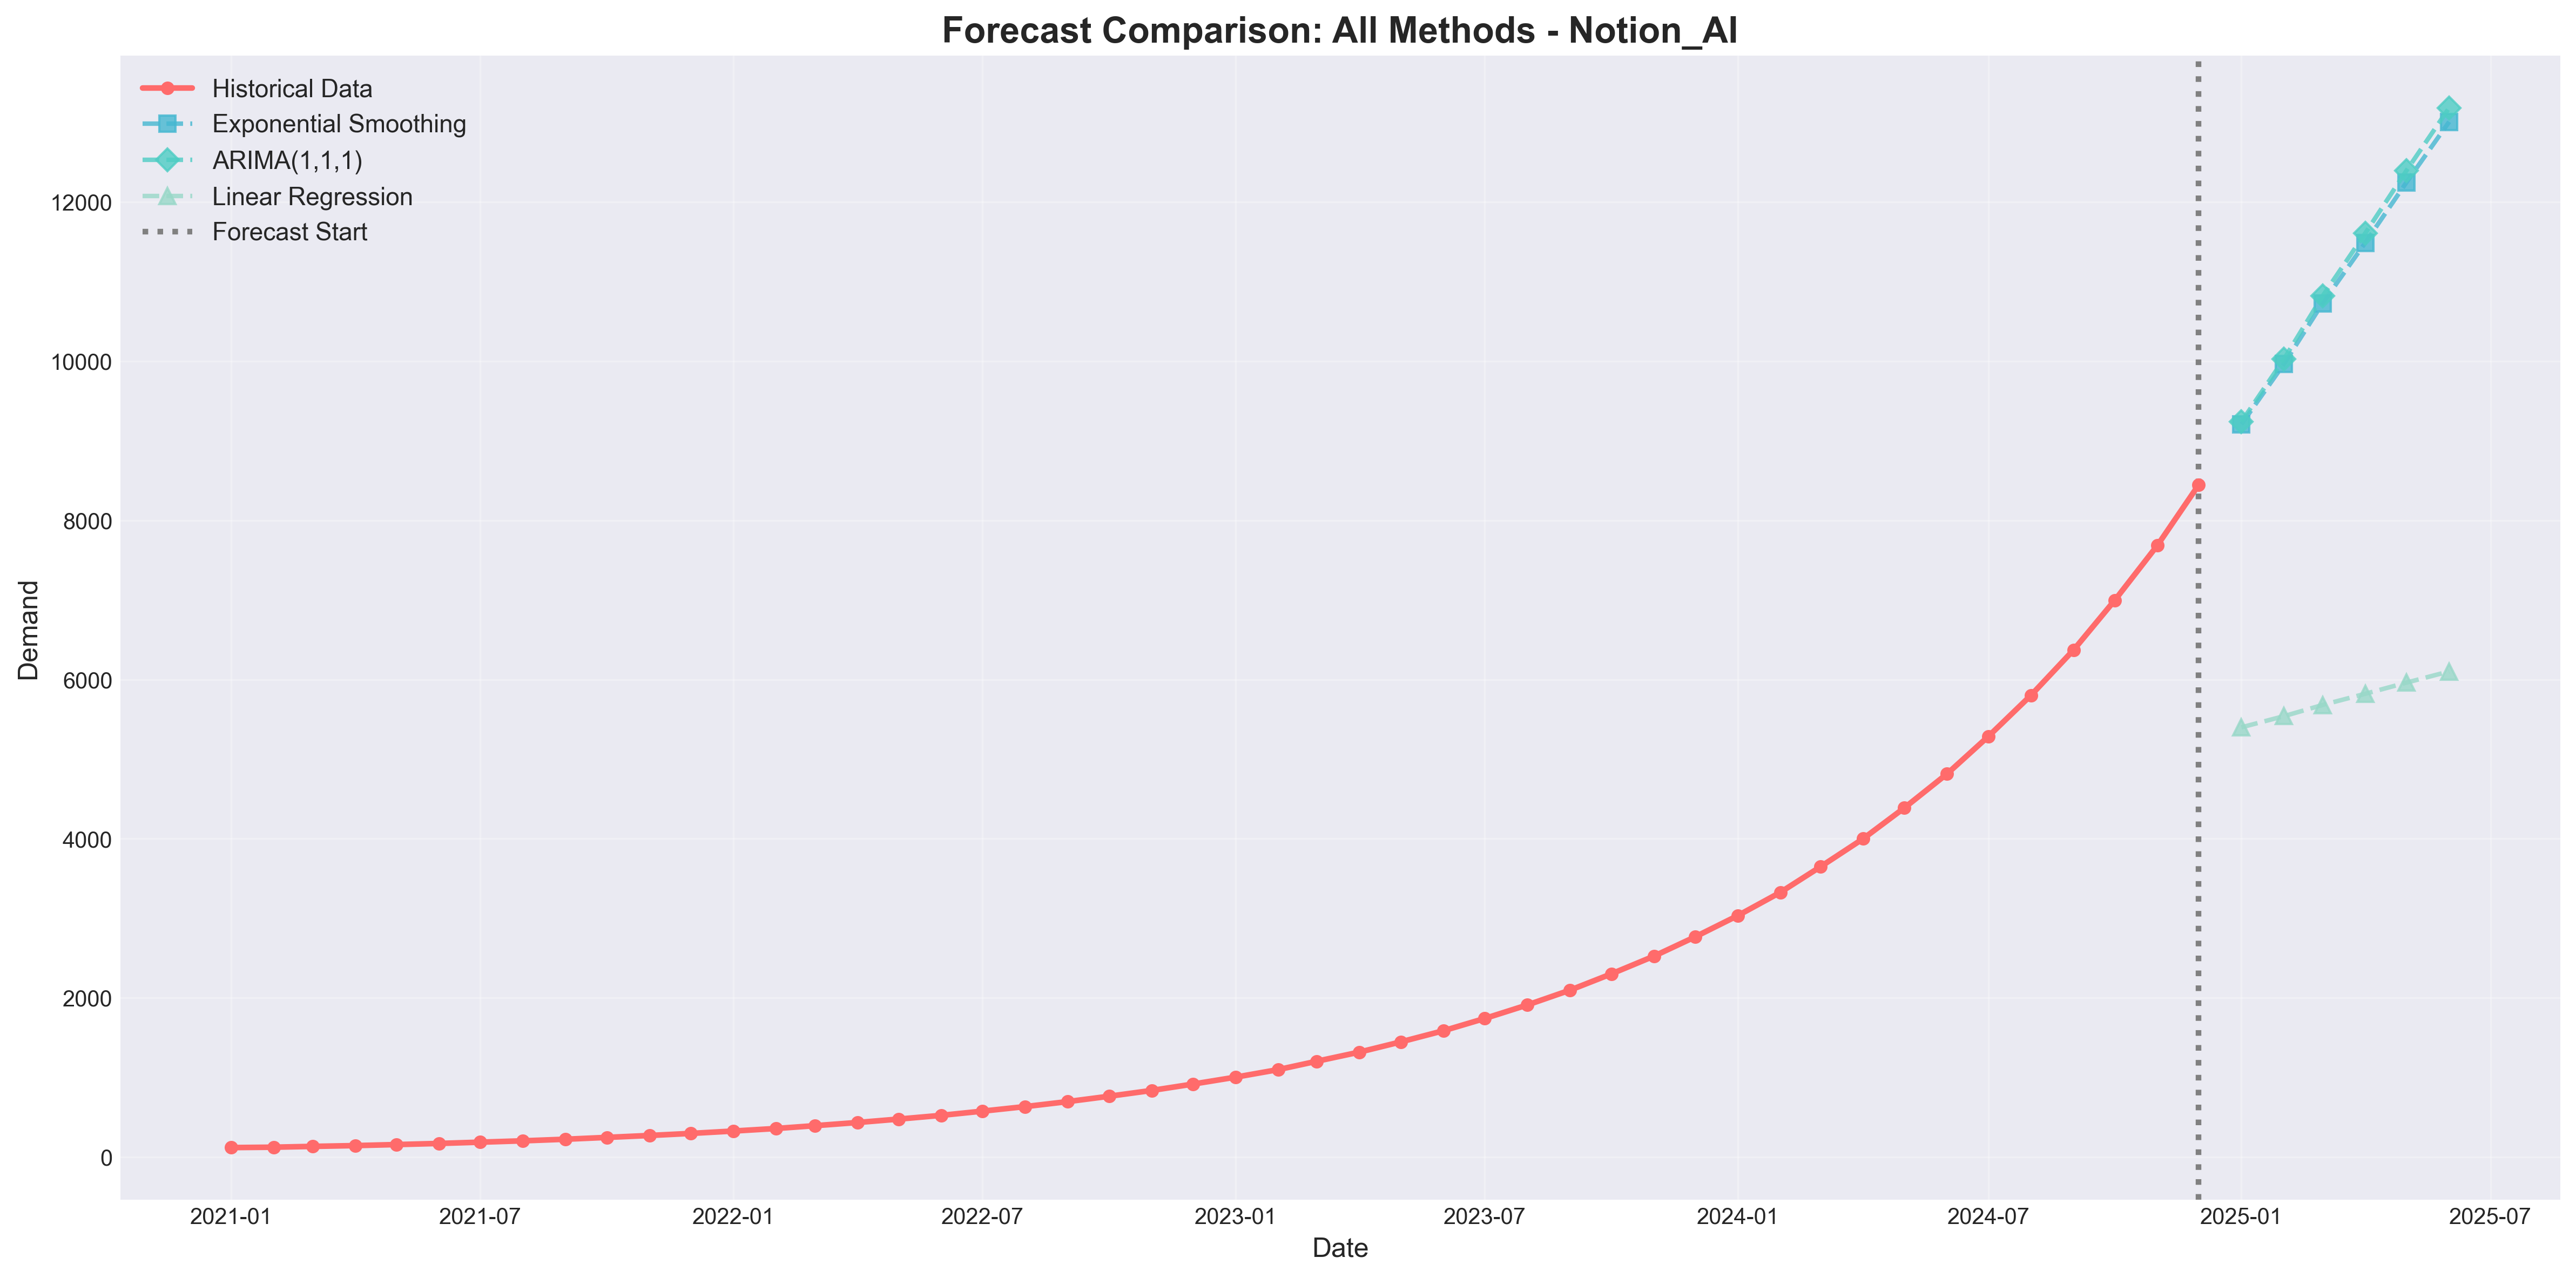
\includegraphics[width=\columnwidth]{figures/fig6_forecast_comparison_all_methods.png}
\caption{Comparison of all three forecasting methods (Exponential Smoothing, ARIMA, and Linear Regression) for Notion AI. While each model produces different predictions, they converge on the same fundamental insight: robust continued growth. This consensus strengthens confidence in resource allocation decisions.}
\label{fig:forecast_comparison}
\end{figure}


\subsection{Hypothesis Validation}
This study hypothesized that forecasted demand patterns can meaningfully inform product design decisions. The analysis provides support for this hypothesis. Features with increasing demand signals—particularly Notion AI—were designated as high priority by the system. The time-series models demonstrated acceptable prediction accuracy, indicating their utility for planning purposes. Most significantly, the system translated numerical outputs into actionable recommendations, bridging the gap between analytical results and design decisions.

\begin{figure}[htbp]
\centering
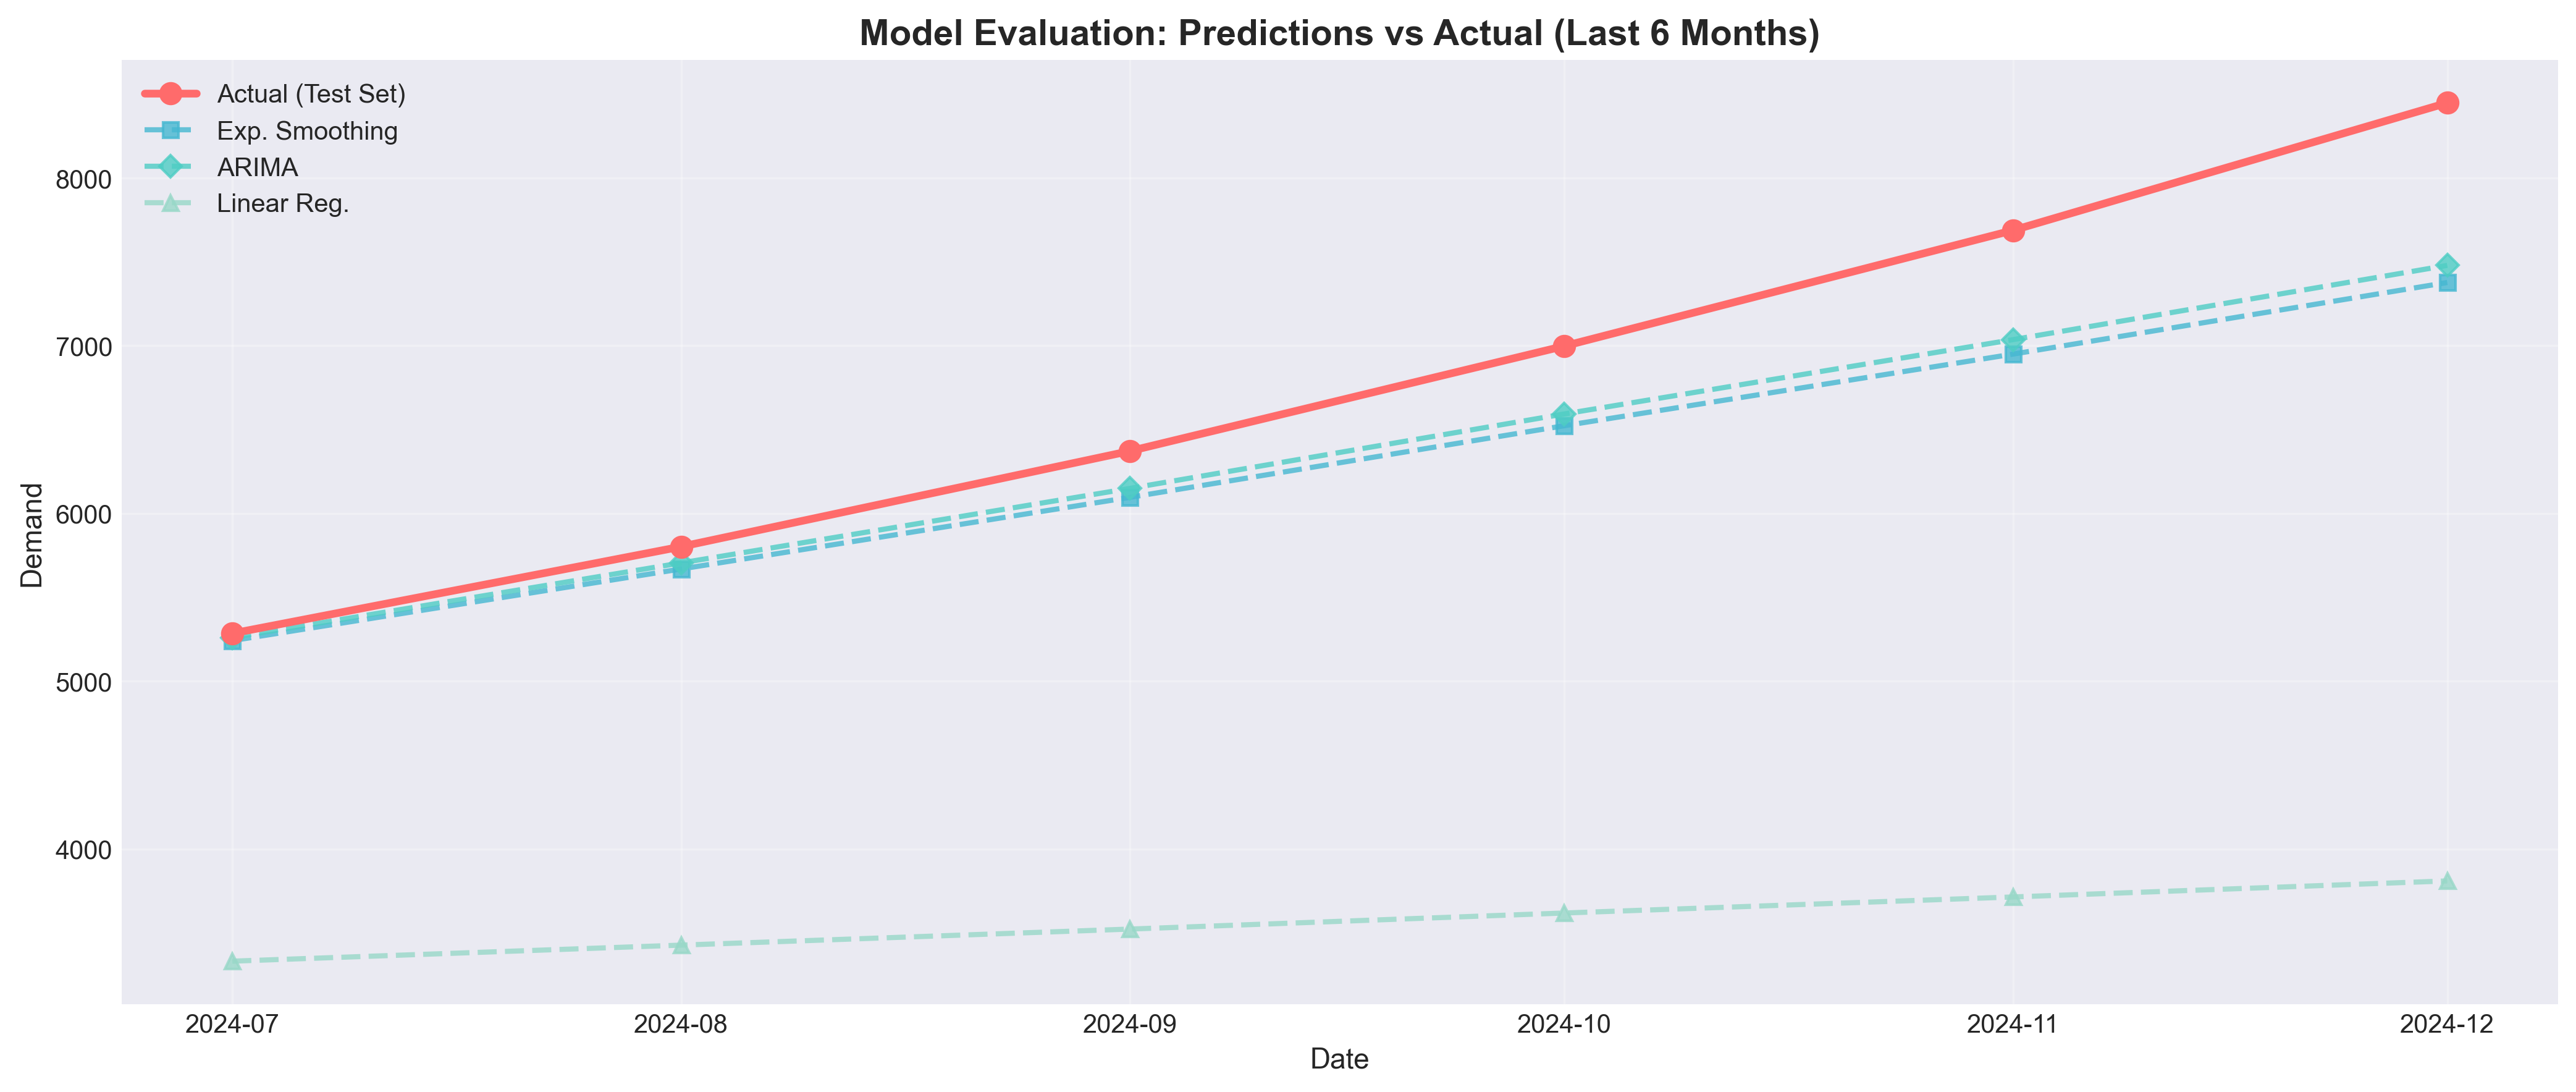
\includegraphics[width=\columnwidth]{figures/fig7_model_evaluation.png}
\caption{Model evaluation on test set (final 6 months of historical data). All three models achieve acceptable accuracy, with predictions closely tracking actual values. This validation confirms model reliability for forward-looking forecasts.}
\label{fig:model_eval}
\end{figure}

Figure \ref{fig:model_eval} demonstrates satisfactory model performance when evaluated against held-out test data, supporting the credibility of forward-looking predictions.

\subsection{Testing and Validation}
Comprehensive testing was conducted rather than relying on informal verification. Unit tests verified that each pipeline component—data cleaning, feature extraction, model training, API responses—functioned as specified. Integration tests confirmed component interoperability. End-to-end smoke tests traversed the complete workflow from data ingestion to chart rendering.

\subsection{Performance Characteristics}
Performance proved sufficient for the intended exploratory analysis. Forecast generation for a single feature typically completes in less than one second, with more complex ARIMA fits requiring several seconds. API response times remained acceptable during development. Scaling to thousands of concurrent users or substantially larger datasets would require optimization investment including caching, asynchronous processing, and database scaling.

\subsection{Challenges Encountered}
Several challenges arose during development.

\textbf{Data source heterogeneity.} Google Trends provides monthly snapshots, reviews include daily timestamps, and some metadata contained gaps. Substantial effort was required to normalize timestamps and address missing data appropriately.

\textbf{Model variability.} Exponential Smoothing performed optimally for some features, ARIMA for others. Rather than selecting a single model, the ensemble approach was adopted with model weights determined by historical performance.

\textbf{Reproducibility requirements.} The analysis would lack credibility without replicability. Datasets were versioned, model artifacts were saved with complete metadata, and all transformation steps were documented.

\subsection{Generated Recommendations}
Based on model outputs, the framework generated the following guidance.

\textbf{Prioritize AI features.} Demand is increasing substantially, warranting investment in discoverability and polish.

\textbf{Maintain template quality.} Templates demonstrate stable popularity—focus on quality maintenance and consider complementary additions.

\textbf{Monitor automation.} Interest is growing but not accelerating rapidly. Investment is warranted but should not divert resources from higher-growth areas.

\begin{figure}[htbp]
\centering
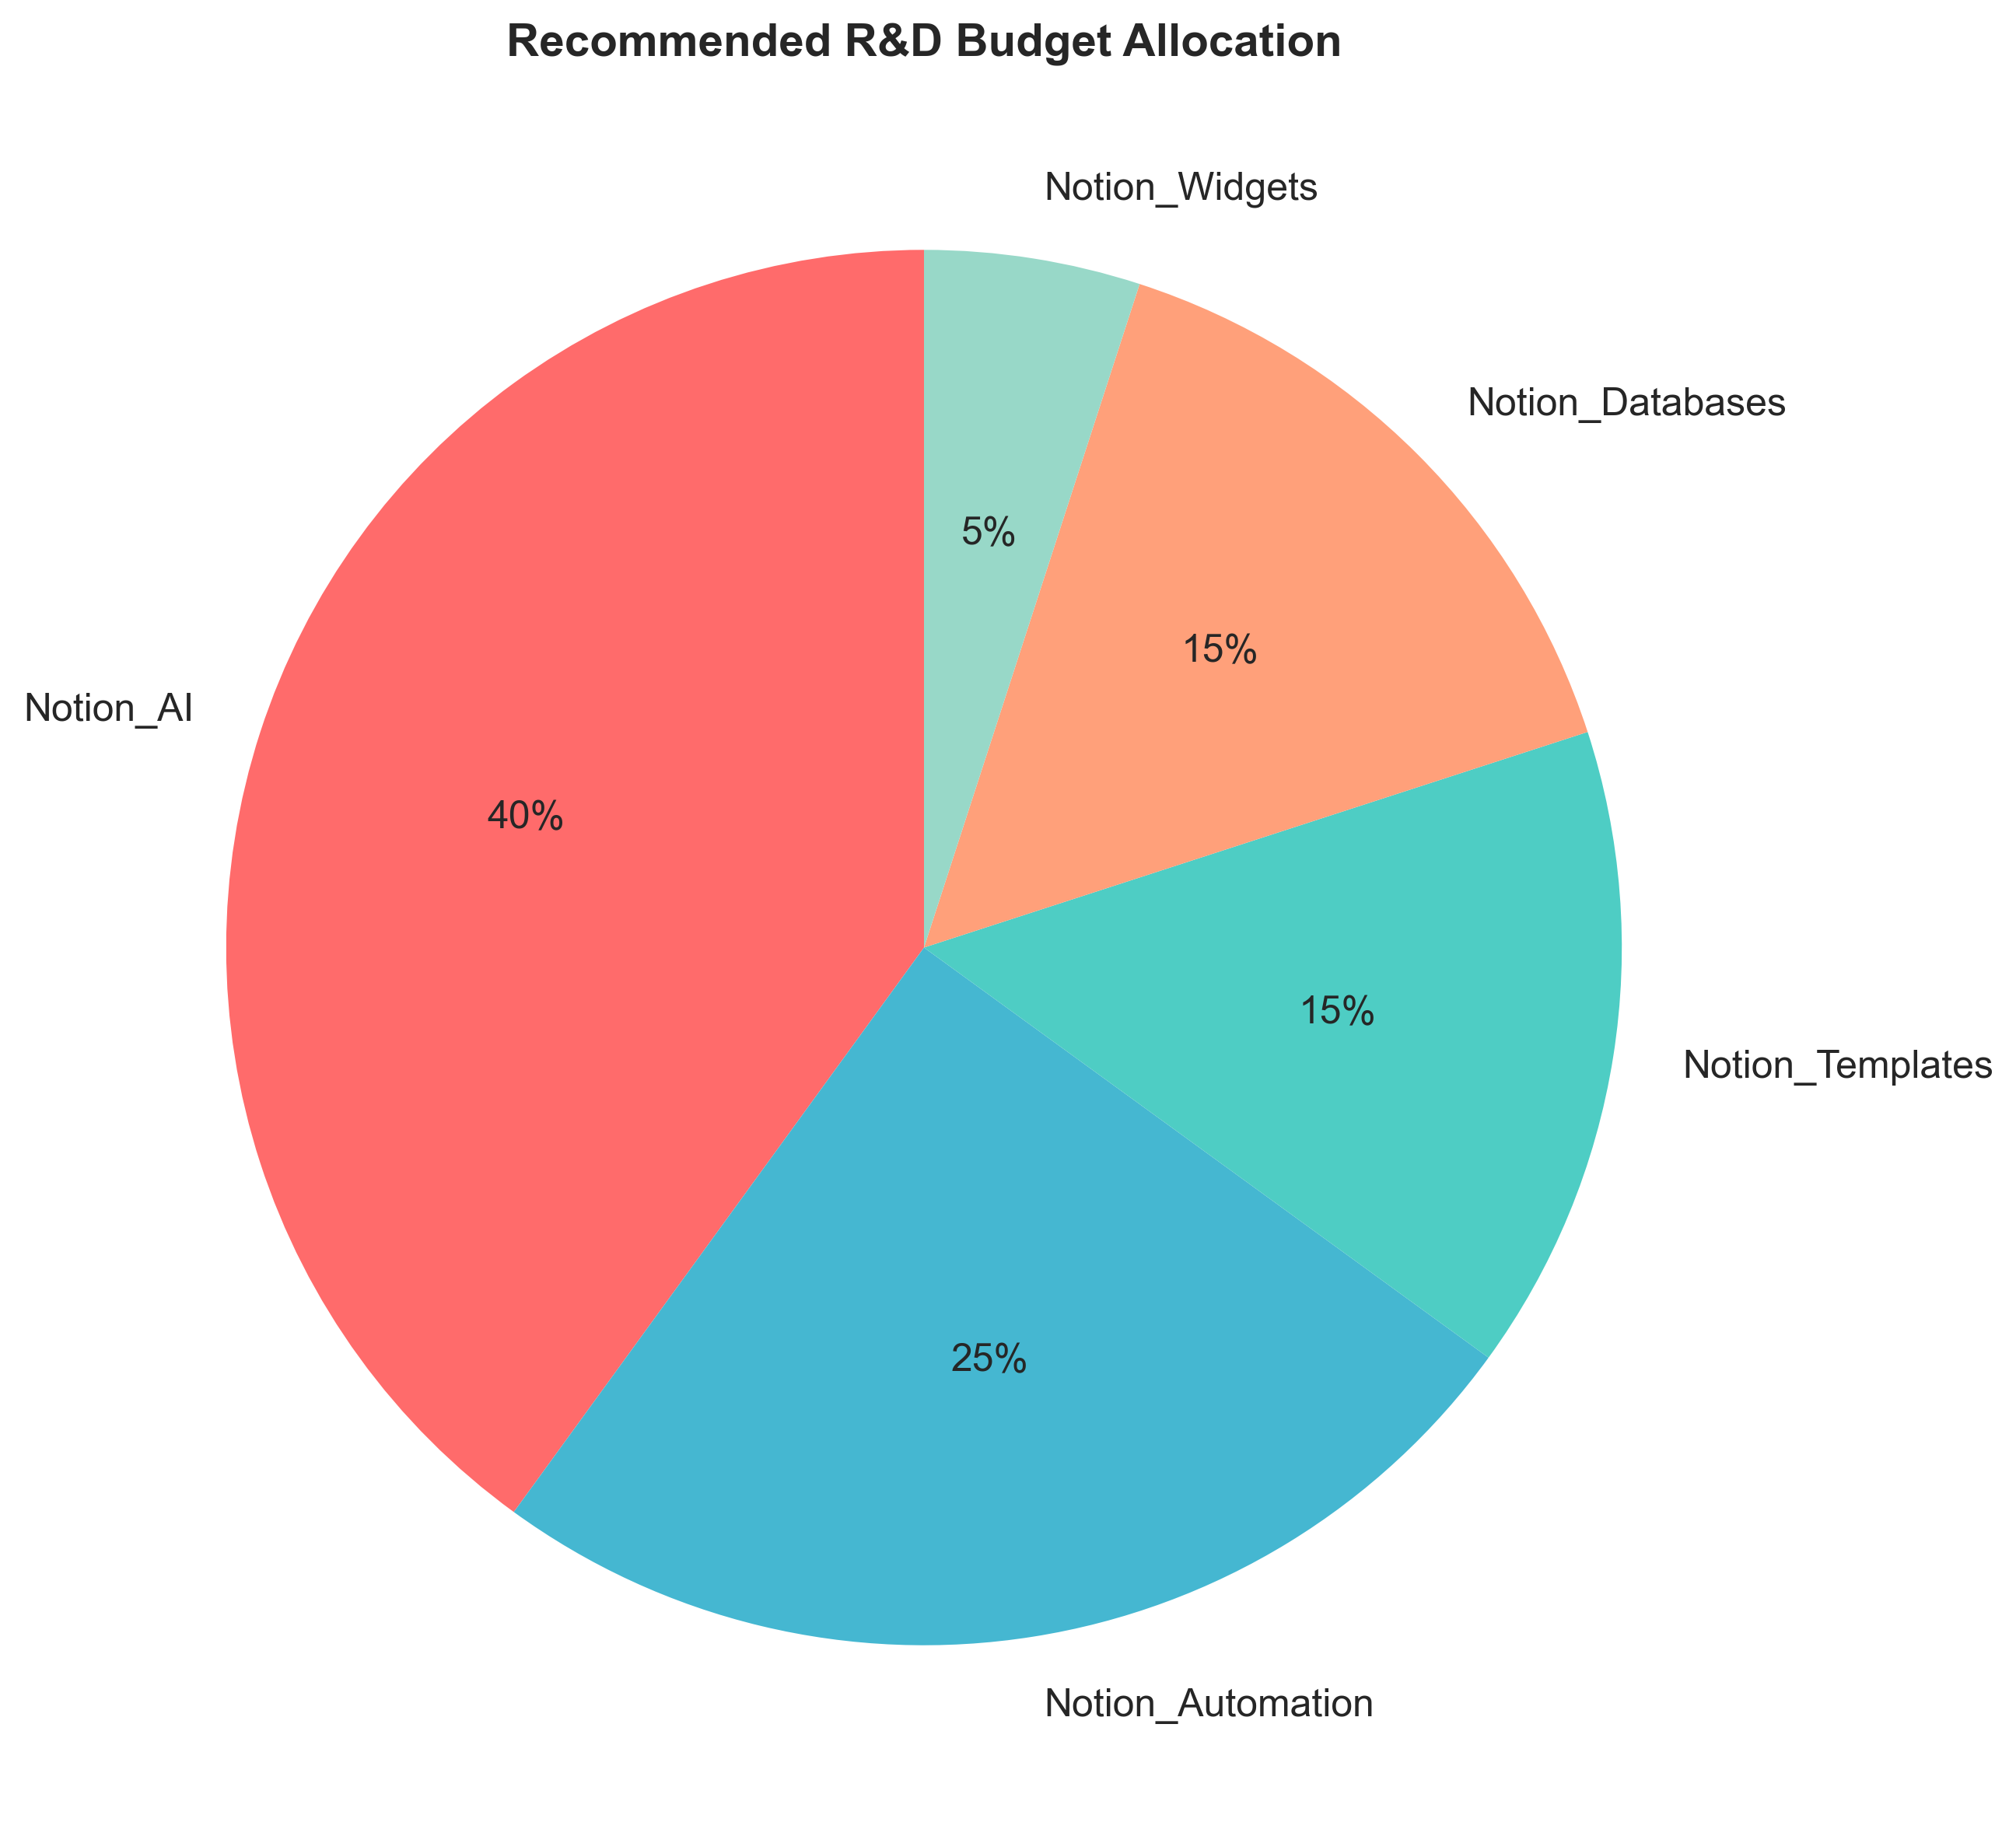
\includegraphics[width=\columnwidth]{figures/fig8a_resource_allocation.png}
\caption{Recommended R\&D budget allocation across features. The distribution prioritizes high-growth features, with Notion AI receiving 40\% based on extraordinary growth potential.}
\label{fig:budget_allocation}
\end{figure}

\begin{figure}[htbp]
\centering
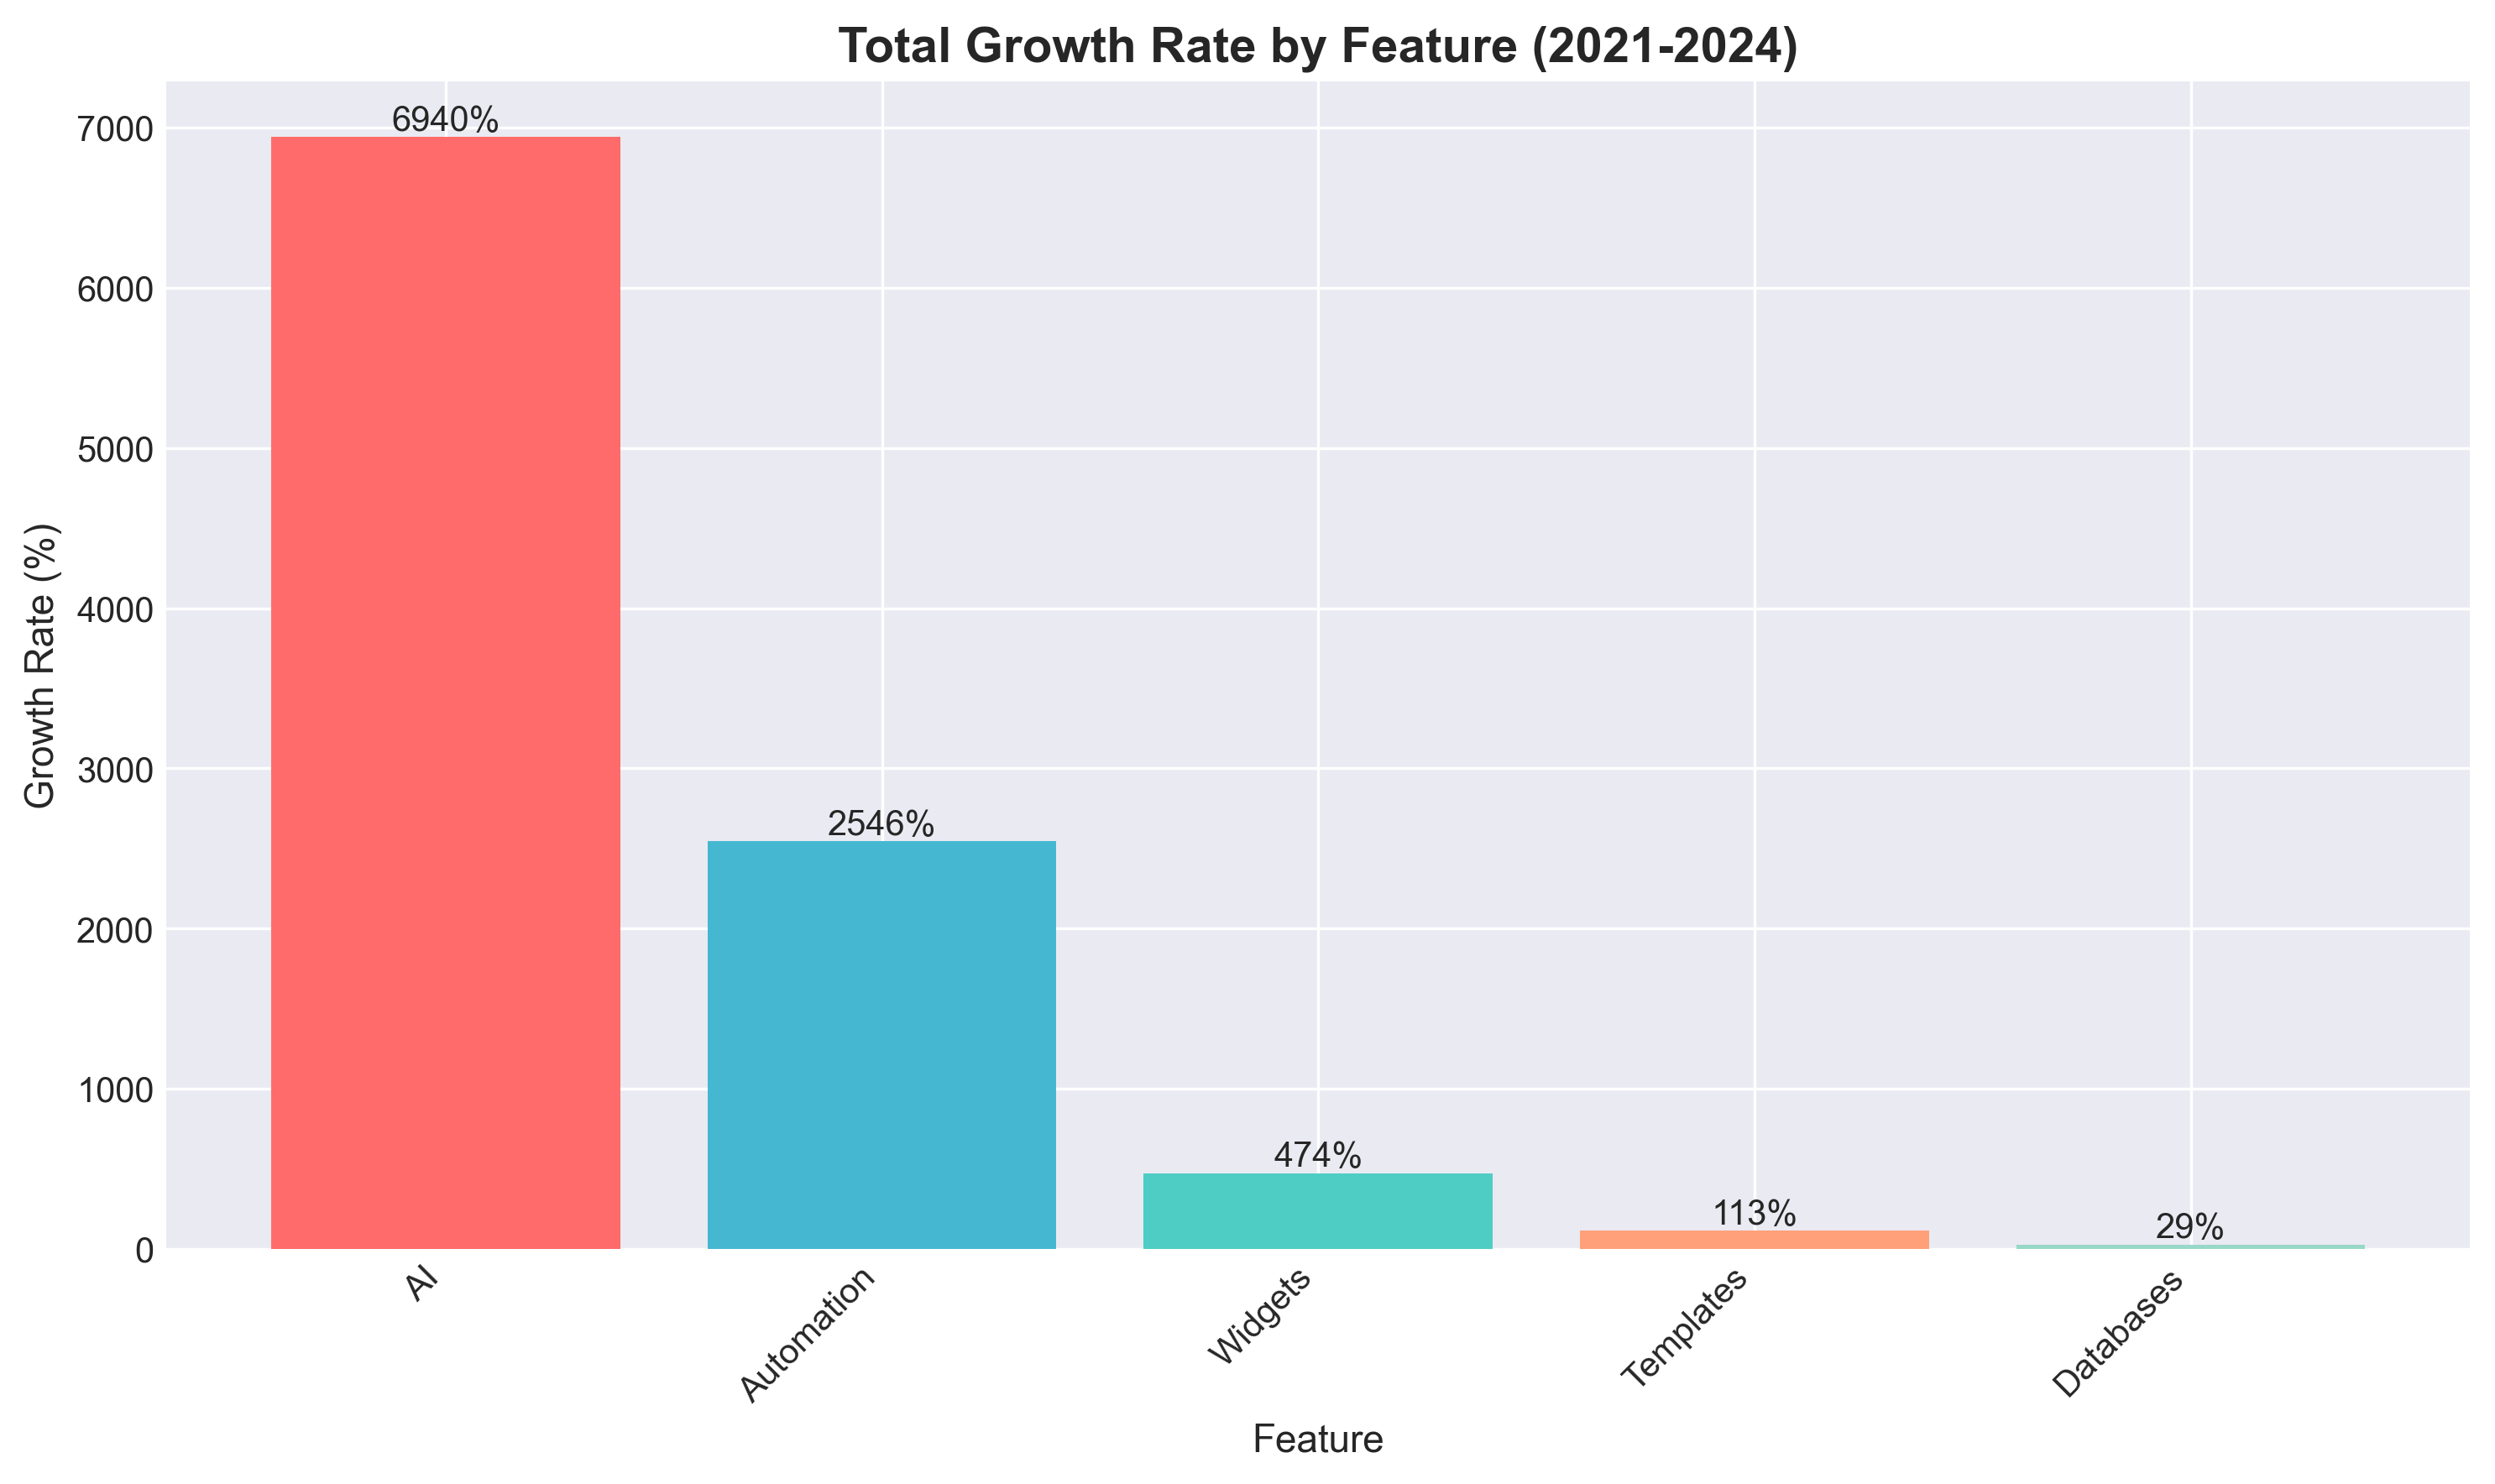
\includegraphics[width=\columnwidth]{figures/fig8b_growth_rates.png}
\caption{Historical growth rates by feature from 2021–2024. Notion AI demonstrates 6940\% growth, justifying prioritization in resource allocation, while Databases shows only 29\% growth as a mature feature.}
\label{fig:growth_rates}
\end{figure}

Figures \ref{fig:budget_allocation} and \ref{fig:growth_rates} translate forecasting insights into strategic recommendations. The allocation chart illustrates recommended R\&D resource distribution, while the bar chart provides growth rate justification. Notion AI receives 40\% of resources based on its 6940\% growth, while mature features such as Databases receive 15\% to maintain stability.

These recommendations demonstrate that the framework achieves its intended objective: connecting demand signals to product decisions.
